\section{Superblock distributions in deployed cryptocurrencies}

We measured the superblock distribution in the mainnet Bitcoin blockchain. Our
results are illustrated in Figure~\ref{fig.btc-superblocks}. As expected,
half the blockchain blocks are $1$-superblocks, $1/4$ of blocks are
$2$-superblocks and generally approximately $2^{-\mu}$ of the blockchain blocks
are $\mu$-superblocks. The horizontal axis denotes the block height, while the
vertical axis denotes the superblock density with respect to the variable
difficulty target of each block, in logarithmic scale.

\begin{figure*}[h]
\begin{center}
  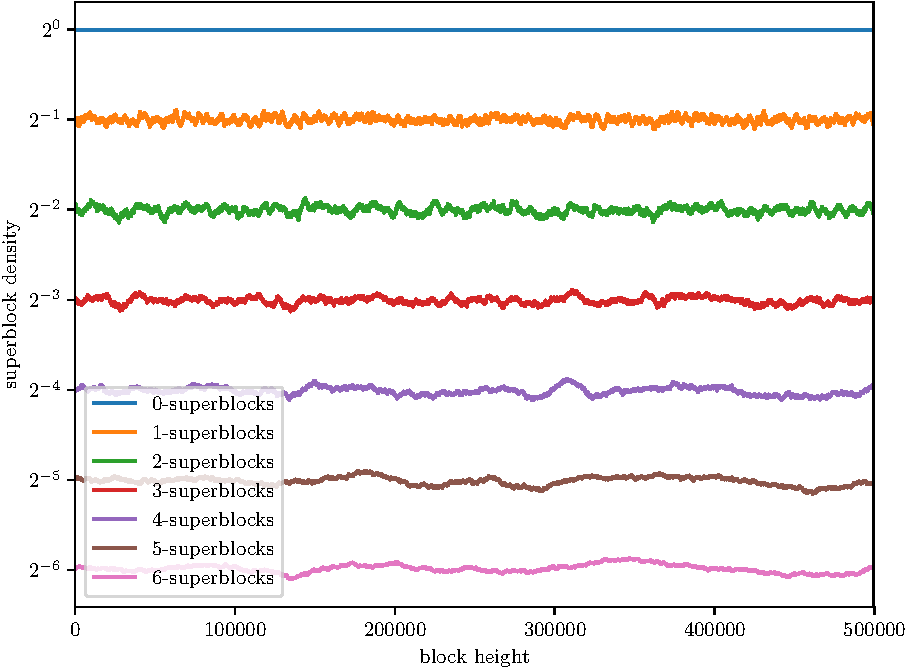
\includegraphics[width=0.95\textwidth]{figures/bitcoin-superblock-distribution.pdf}
  \caption{Distribution of block levels in Bitcoin. Superblocks are with
    respect to variable difficulty targets. Shaded area indicates
    $\pm1\sigma$.}
  \label{fig.btc-superblocks}
  \end{center}
\end{figure*}

We performed these measurements as follows. We downloaded the whole bitcoin
blockchain from the Genesis block up to the current tip of the blockchain
(at the time of writing $563{,}451$). We then plotted the density for each level $\mu = 0 \dots 6$. For the particular level, we traversed the blockchain using
a sliding window of $1000 (2^\mu) + 1$ blocks. Within that sliding window, we
measured how many blocks of level $\mu$ exist, and plotted the ratio of the
count of these superblocks within the window to the window size. The plot for
level $0$ is flat, as all blocks are $0$-superblocks. The high-frequency erratic
behavior is due to the probabilistic nature of block generation. We conjecture
that lower frequency patterns, especially those aligned between multiple levels,
are due to difficulty adjustment which incorrectly predicted the underlying
computational power for a given epoch (e.g., due to rapidly changing costs in
mining hardware or cryptocurrency prices).
